\documentclass[oneside, 11pt]{article}

\usepackage[T1]{fontenc}
\usepackage[utf8]{inputenc}
\usepackage[english]{babel}

\usepackage{fouriernc}
\usepackage[detect-all, binary-units, separate-uncertainty=true,
            per-mode=symbol, retain-explicit-plus, retain-unity-mantissa=false]{siunitx}

\usepackage{setspace}
\setstretch{1.2}

\setlength{\parskip}{\smallskipamount}
\setlength{\parindent}{0pt}

\usepackage[headheight=14pt]{geometry}
\geometry{marginparwidth=0.5cm, verbose, a4paper, tmargin=3cm, bmargin=3cm,
          lmargin=2cm, rmargin=2cm}

\usepackage{float}

\usepackage[fleqn]{amsmath}
\numberwithin{equation}{section}
\numberwithin{figure}{section}

\usepackage{graphicx}
\graphicspath{{images/}{../../../images/}}

\usepackage{tikz}
\usetikzlibrary{shapes}
\usetikzlibrary{plotmarks}

\newcounter{Exercise}
\setcounter{Exercise}{1}
\usepackage{xcolor}
\definecolor{shadecolor}{gray}{0.9}
\usepackage{framed}
\usepackage{caption}

\usepackage{url}


\usepackage{fancyhdr}
\pagestyle{fancy}
\fancyhf{}
\rhead{\thepage}
\renewcommand{\footrulewidth}{0pt}
\renewcommand{\headrulewidth}{0pt}

\fancypagestyle{firststyle}
{
    \fancyhf{}
    \rhead{\thepage}
    \cfoot{
\includegraphics[height=30pt]{HiSPARClogo}}
    \rfoot{
\includegraphics[height=25pt]{CCbysa}}
    \lfoot{
\includegraphics[height=30pt]{NIKHEFlogo}}
    \renewcommand{\footskip}{50pt}
    \renewcommand{\footrulewidth}{0.1pt}
    \renewcommand{\headrulewidth}{0pt}
}

\newcommand{\figref}[1]{Figuur~\ref{#1}}

\newcommand{\hisparc}{\textsmaller{HiSPARC}\xspace}
\newcommand{\kascade}{\textsmaller{KASCADE}\xspace}
\newcommand{\sapphire}{\textsmaller{SAPPHiRE}\xspace}
\newcommand{\jsparc}{\textsmaller{jSparc}\xspace}
\newcommand{\hdf}{\textsmaller{HDF5}\xspace}
\newcommand{\aires}{\textsmaller{AIRES}\xspace}
\newcommand{\csv}{\textsmaller{CSV}\xspace}
\newcommand{\python}{\textsmaller{PYTHON}\xspace}
\newcommand{\corsika}{\textsmaller{CORSIKA}\xspace}
\newcommand{\labview}{\textsmaller{LabVIEW}\xspace}
\newcommand{\daq}{\textsmaller{DAQ}\xspace}
\newcommand{\adc}{\textsmaller{ADC}\xspace}
\newcommand{\hi}{\textsc{h i}\xspace}
\newcommand{\hii}{\textsc{h ii}\xspace}
\newcommand{\mip}{\textsmaller{MIP}\xspace}
\newcommand{\hisparcii}{\textsmaller{HiSPARC II}\xspace}
\newcommand{\hisparciii}{\textsmaller{HiSPARC III}\xspace}

\DeclareSIUnit{\electronvolt}{\ensuremath{\mathrm{e\!\!\:V}}}

\DeclareSIUnit{\unitsigma}{\ensuremath{\sigma}}
\DeclareSIUnit{\mip}{\textsmaller{MIP}}
\DeclareSIUnit{\adc}{\textsmaller{ADC}}

\DeclareSIUnit{\gauss}{G}
\DeclareSIUnit{\parsec}{pc}
\DeclareSIUnit{\year}{yr}




%document details
\author{N.G. Schultheiss \\ translated and adapted by K. Schadenberg}
\date{}
\title{Lenses}


\begin{document}
\maketitle

\section{Introduction}
This module `Lenses' summarizes and extends your basic knowledge about lenses. After this module you can proceed with the modules `Telescopes' or `Grinding lenses'. When you completed all these modules you should be able to make your own telescope with the help of the module `Making your own telescope' and explain how it works.

\section{Ray diagram}
This sections briefly summarises the knowledge of lenses from key stage 3 and 4.

One can use the thin lens formula
\begin{equation}
\frac{1}{f}=\frac{1}{i}+\frac{1}{o} \label{eg:lens_equation}
\end{equation}
to calculate the focal length $f$, the image distance $i$, or the object distance $o$ when the other two variables are known.\footnote{You might have used different symbols to denote the distance to the object and image: $v$ instead of $i$ and $u$ instead of $o$.}

The equation for linear magnification
\begin{equation}
M = - \frac{i}{o} = \frac{\mbox{Height image}}{\mbox{Height object}}
\end{equation}
can be used to calculate the magnification. But also one of the four variables if the other three are known.

The image of an object can be constructed using three special construction lines in the ray diagram:
\begin{itemize}
\item One ray of light straight through the centre of the lens without refraction.
\item One ray of light travelling parallel to the main axis of the lens before the lens that gets refracted towards and passes through the focal point after the lens.
\item One ray of light that passes through the focal point before the lens and continues parallel to the main axis after the lens.
\end{itemize}

\begin{figure}\begin{center}
\begin{picture}(0,0)%
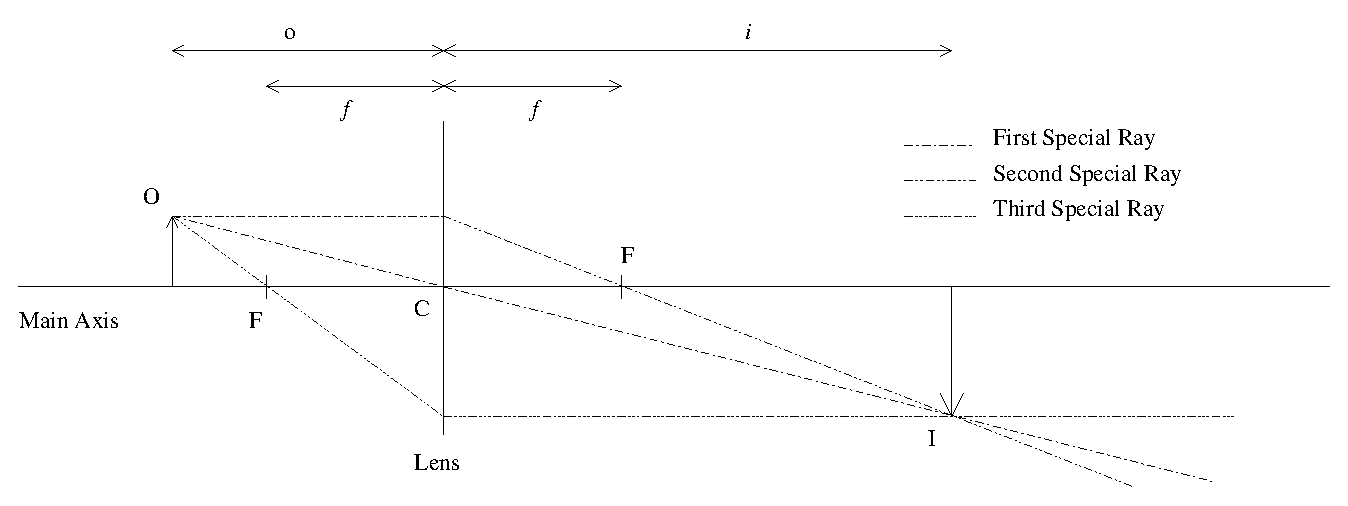
\includegraphics[scale=0.7]{construction_ray_diagram}%
\end{picture}%
\setlength{\unitlength}{4144sp}%
%
\begingroup\makeatletter\ifx\SetFigFont\undefined%
\gdef\SetFigFont#1#2#3#4#5{%
  \reset@font\fontsize{#1}{#2pt}%
  \fontfamily{#3}\fontseries{#4}\fontshape{#5}%
  \selectfont}%
\fi\endgroup%
\begin{picture}(10017,3597)(1516,-4393)
\end{picture}%
\caption{Constructing a ray diagram using three special lines.}\label{fig:ray_diagram}
\end{center}\end{figure}

In figure \ref{fig:ray_diagram} all distances and lines are shown. Notice that points are indicated using capitals while distances are in lower case.
\begin{enumerate}[ ]
\item C: Optical centre (Centre of the lens)
\item F: Focal point
\item O: Point of light, the object radiates (or reflects) light at every point
\item I: Image point
\end{enumerate}

The three lines intersect each other at the some point some distance behind the lens. Here we find our image of the object. Do you remember where the image of the object is when the lines do not intersect after the lens?

\section{How a lens works}
Lenses work because of interaction between light and matter. When there is no matter present light will move with the speed of light in vacuum $c$.\footnote{Sometimes only `speed of light' is mentioned in texts, from the context one needs to deduce if this is the speed of light in vacuum or not.} The unit of distance, the metre, is defined according to the speed of light, therefore the speed of light is by definition exactly $c=299792458~m~s^{-1} $.

From experience we know that light only travels through transparent materials. Inside the material the light will always move slower than in vacuum. In water the speed is roughly 3/4 of the speed of light (in vacuum), in glass 2/3. The difference in speed is the cause of refraction.

\begin{shaded}
\textbf{Exercise \theExercise \stepcounter{Exercise}} : In the module `Mirrors' the Huygens principle was introduced. Explain what happens to the distance between the wave fronts when a beam of light goes from water to vacuum (where no matter is present).\end{shaded}

\begin{figure}\begin{center}
\begin{picture}(0,0)%
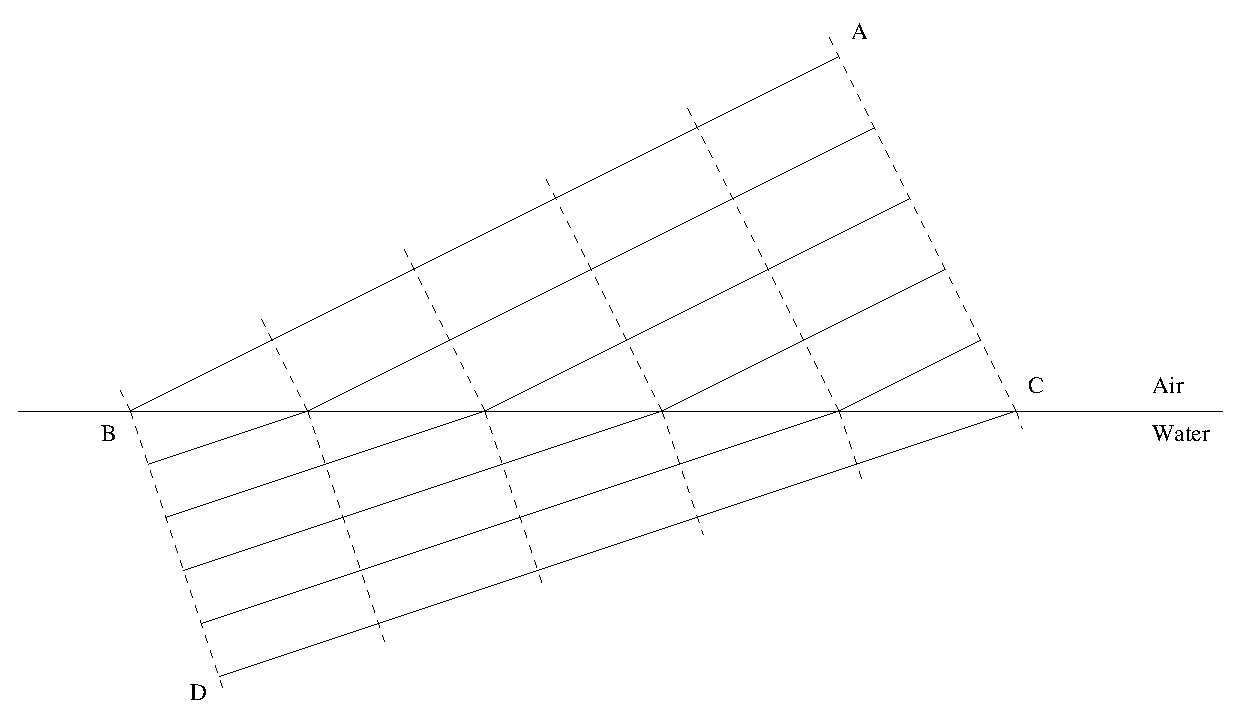
\includegraphics[scale=0.75]{refraction}%
\end{picture}%
\setlength{\unitlength}{4144sp}%
%
\begingroup\makeatletter\ifx\SetFigFont\undefined%
\gdef\SetFigFont#1#2#3#4#5{%
  \reset@font\fontsize{#1}{#2pt}%
  \fontfamily{#3}\fontseries{#4}\fontshape{#5}%
  \selectfont}%
\fi\endgroup%
\begin{picture}(9220,5220)(-326,-5251)
\end{picture}%
\caption{Refraction at an air/water interface.}\label{fig:interface}
\end{center}\end{figure}

In figure \ref{fig:interface} two large triangles are shown, $\Delta$ABC and $\Delta$BCD. Clearly the segment (BC) is present in both triangles. We know from the module `Mirrors' that the wave front is always perpendicular to the wave beam: \angle BAC = \angle BDC = 90$^{\circ}$

\begin{shaded}
\textbf{Exercise \theExercise \stepcounter{Exercise}} : Explain how to determine the value of $\sin$(\angle ABC).\end{shaded}
\begin{shaded}
\textbf{Exercise \theExercise \stepcounter{Exercise}} : Explain how to determine the value of $\sin$(\angle BCD).\end{shaded}
\begin{shaded}
\textbf{Exercise \theExercise \stepcounter{Exercise}} : Show that: \begin{equation} \frac{\sin(\angle ABC)}{\sin(\angle BCD)} = \frac{(AC)}{(BD)} \end{equation}\end{shaded}
\begin{shaded}
\textbf{Exercise \theExercise \stepcounter{Exercise}} : Explain than the ratio $\frac{(AC)}{(BD)}$ is equal to the ratio between the speeds of light.\end{shaded}

The ration between the speeds of light is called the refractive index, in this case $n_{air \rightarrow water}$.

\begin{shaded}
\textbf{Exercise \theExercise \stepcounter{Exercise}} : Show that the angles \angle ABC and \angle BCD are equal to the angle of incidence $i$ (between the incident ray and the surface normal) and the angle of refraction $r$ (between the refracted ray and the surface normal).\end{shaded}
\begin{shaded}
\textbf{Exercise \theExercise \stepcounter{Exercise}} : Explain the following formula\footnotemark: \begin{equation} n = \frac{\sin(i)}{\sin(r)}\end{equation}\end{shaded}
\footnotetext{The formula is known as Snell's Law, named after the Dutch scientist Willebrord Snel van Royen (1580-1626). In his time Latin names where the norm so he is better known as Snellius. The relationship he described was already known but he was the first to capture it in a mathematical notation. We do not use Snellius his original notation but a modified form by Ren\'e Descartes, therefore the French call the law Descartes Law.}

\section{Construction of refraction at plane and spherical surfaces}
Drawing many wave fronts and beams can be very cumbersome, we will therefore use two different construction techniques to draw refraction at plane and spherical surfaces. These techniques allow us to follow a single ray of light; ray tracing. 

\begin{figure}\begin{center}
\begin{picture}(0,0)%
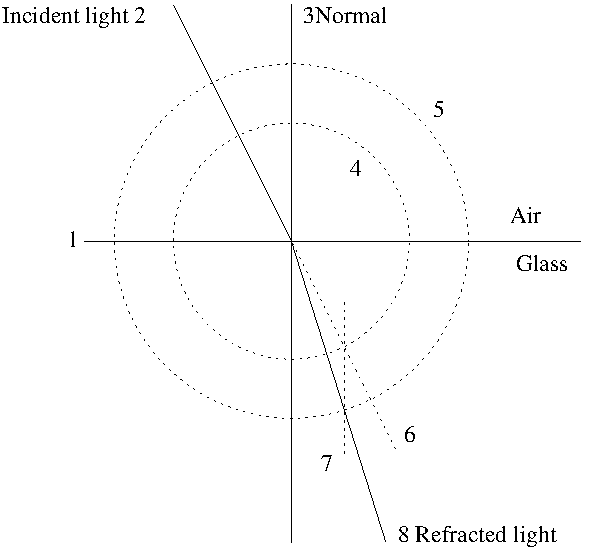
\includegraphics{plane}%
\end{picture}%
\setlength{\unitlength}{4144sp}%
%
\begingroup\makeatletter\ifx\SetFigFont\undefined%
\gdef\SetFigFont#1#2#3#4#5{%
  \reset@font\fontsize{#1}{#2pt}%
  \fontfamily{#3}\fontseries{#4}\fontshape{#5}%
  \selectfont}%
\fi\endgroup%
\begin{picture}(4491,4204)(571,-3599)
\end{picture}%
\caption{Refraction at a flat surface.}\label{fig:refraction_plane}
\end{center}\end{figure}

Take a look at figure~\ref{fig:refraction_plane}. In this figure there are a couple of numbers. These relate to the following steps in ray tracing:
\begin{enumerate}[1.]
\item Draw the surface between both materials (interface), in this case air and glass.
\item Draw the incident ray.
\item Draw the surface normal at the intersection of the incident ray and the surface. Remember that the surface normal is always perpendicular to the surface.
\item Draw a circle with the intersection as its centre. We are free to choose the radius of the circle, in this case we chose 1.5 cm.
\item Draw a second concentric circle (having the same midpoint) with a radius $N$ times larger than the previous circle, in this case 2.25 cm.
\item Extend the incident ray with a dotted line.
\item Draw a dotted line parallel to the surface normal starting at the intersection of the first circle (4) and the previous dotted line (6).
\item Draw the refracted line, starting at the end of the incident ray and through the intersection of the second circle (5) and the previous line (7).
\end{enumerate}

\begin{shaded}
\textbf{Exercise \theExercise \stepcounter{Exercise}} : A ray of light hits a diamond at an angle of $i=25^{\circ}$. Construct the refracted ray, $n_{air \rightarrow diamond} = 2.417.$\end{shaded}

When constructing refractions at spherical surfaces we need three concentric circles.
\begin{figure}\begin{center}
\begin{picture}(0,0)%
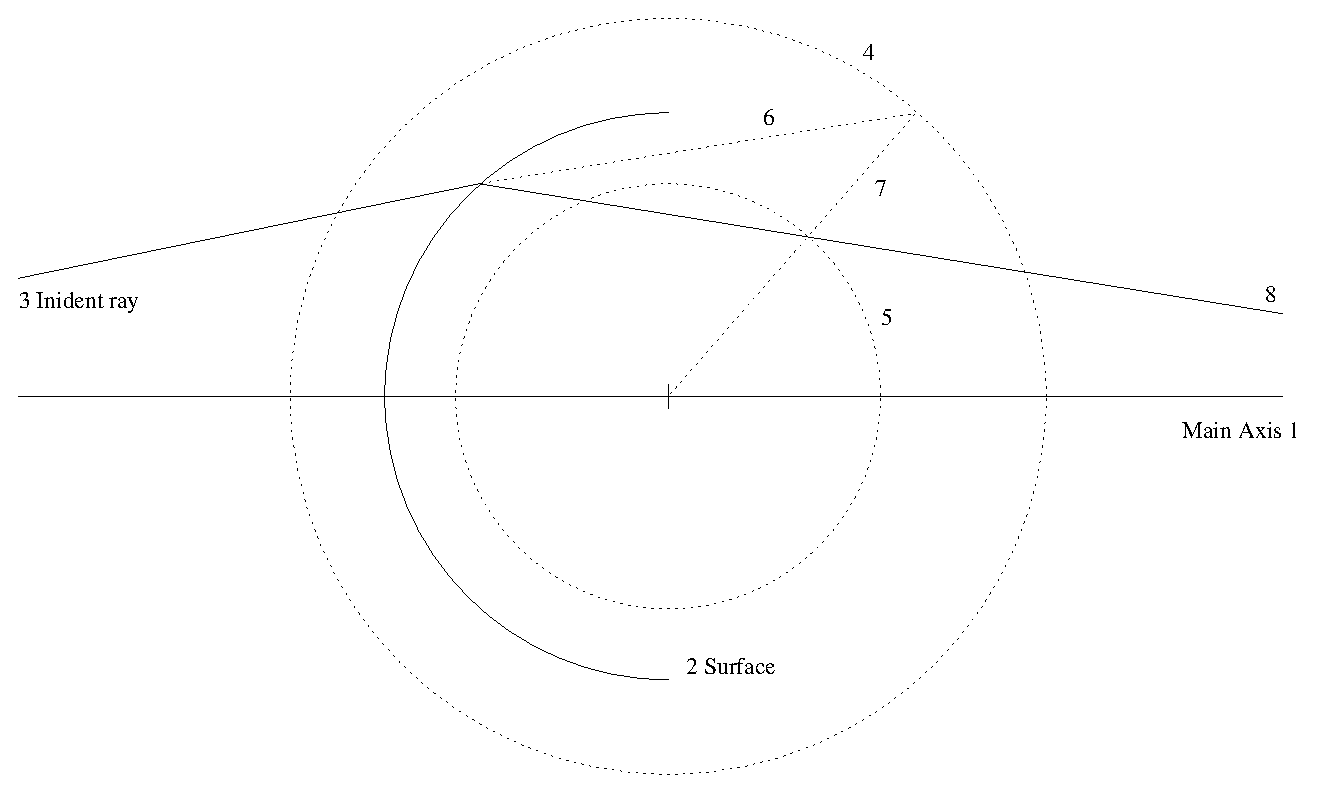
\includegraphics[scale=0.72]{sphere}%
\end{picture}%
\setlength{\unitlength}{4144sp}%
%
\begingroup\makeatletter\ifx\SetFigFont\undefined%
\gdef\SetFigFont#1#2#3#4#5{%
  \reset@font\fontsize{#1}{#2pt}%
  \fontfamily{#3}\fontseries{#4}\fontshape{#5}%
  \selectfont}%
\fi\endgroup%
\begin{picture}(9971,3774)(-374,-5288)
\end{picture}%
\caption{Refraction at a curved surface.}\label{fig:refraction_curve}
\end{center}\end{figure}
The procedure is now as follows (see figure \ref{fig:refraction_curve}):
\begin{enumerate}[1.]
\item Draw the main axis.
\item Draw the spherical surface. In this example we used $r=3.6$~cm. Take care to mark the centre of the sphere.
\item Draw the incident ray.
\item Draw an auxiliary circle with a radius $N$ (refractive index) times as large as the radius of the surface, in this example $r=4.8$~cm.
\item Draw a second auxiliary circle with a radius $N$ (refractive index) times as smaller than the radius of the surface, in this example $r=2.7$~cm.
\item Continue the incident ray to the outermost circle (4) as if it was not refracted.
\item Draw a line from this intersection to the centre of the circles.
\item Draw the refracted ray from the reflecting surface towards the intersection of the previous line (7) and the inner circle (5).
\end{enumerate}

Sometimes we are not interested in the exact path of light but only in the focal length of a lens. It that case we can use the Lens-Maker's Formula\footnote{Here we use an approximation of the Lens-Makers Formula only valid for thin lenses.}:
\begin{equation}
P=\frac{1}{f}=(n-1)\left( \frac{1}{R_1} - \frac{1}{R_2} \right)
\end{equation}
$P$ is the power of the lens, a different way to report its focal length $f$, $n$ is the refractive index, $R_1$ and $R_2$ are the radii of the curvature of the lens. Take care, convention dictates that lengths to the right are positive and to the left are negative. A lens with two convex sides (biconvex) has one positive radius $R_1$, from the surface to the centre, and one negative radius $R_2$, also from the surface to the centre.

If we know the dimensions and the refractive index of the lens we can calculate the focal length. A lens with $R_1=10.0$~cm, $R_2=5.0$~cm, and $n_{lens}=1.50$ will have the following focal length:
\begin{align*}
\frac{1}{f} &= (1.50 - 1) \left( \frac{1}{0.10} - \frac{1}{-0.050} \right) \\
\frac{1}{f} &= (0.50)(10+20) \\
\frac{1}{f} &= 15 \\
f &= \frac{1}{15}~\mbox{m}
\end{align*}

\begin{figure}\begin{center}
\begin{picture}(0,0)%
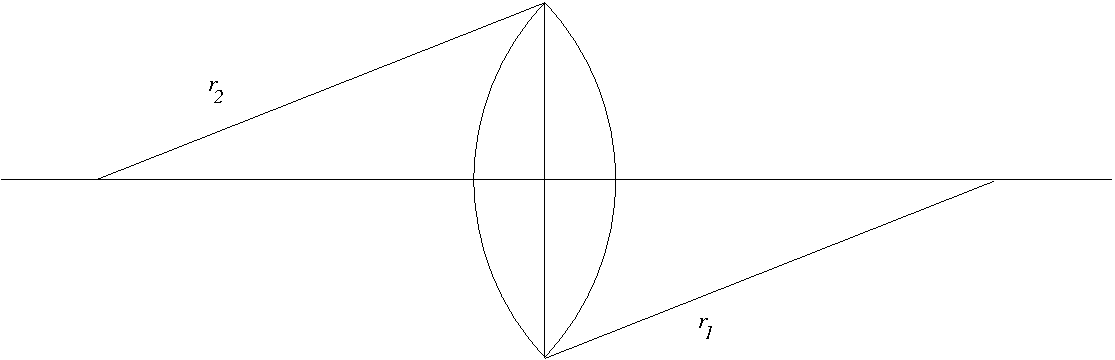
\includegraphics[scale=0.84]{lens}%
\end{picture}%
\setlength{\unitlength}{4144sp}%
%
\begingroup\makeatletter\ifx\SetFigFont\undefined%
\gdef\SetFigFont#1#2#3#4#5{%
  \reset@font\fontsize{#1}{#2pt}%
  \fontfamily{#3}\fontseries{#4}\fontshape{#5}%
  \selectfont}%
\fi\endgroup%
\begin{picture}(8484,2734)(2239,-5663)
\end{picture}%
\caption{A lens.}\label{fig:a_lens}
\end{center}\end{figure}

\begin{shaded}
\textbf{Exercise \theExercise \stepcounter{Exercise}} : Calculate the focal length of plano-convex lens using the following parameters; $R_1=\infty$, $R_2=4.0$~cm, and $n_{lens}=2.0$.\end{shaded}
\begin{shaded}
\textbf{Exercise \theExercise \stepcounter{Exercise}} : Check your previous calculation by drawing the lens and two rays running parallel to the main axis placed at a distance of 1.0 and 2.0 cm.\end{shaded}
\begin{shaded}
\textbf{Exercise \theExercise \stepcounter{Exercise}} : Does the construction result in a clear focal point? If so, what is the focal distance?\end{shaded}

Even if you work very carefully the focal point will not be a perfect spot. Our lens is not perfect. The specific lens error in this case is spherical aberration.

\end{document}